\documentclass[9pt,aspectratio=169]{beamer}
\usetheme[progressbar=frametitle, block=fill]{metropolis}

\usepackage{fontspec}
\setsansfont{FiraSans}[
  Path=/usr/local/texlive/2026basic/texmf-dist/fonts/opentype/public/fira/,
  Extension=.otf,
  UprightFont=*-Light,
  BoldFont=*-Regular,
  ItalicFont=*-LightItalic,
  BoldItalicFont=*-Italic
]
\setmainfont{FiraSans}[
  Path=/usr/local/texlive/2026basic/texmf-dist/fonts/opentype/public/fira/,
  Extension=.otf,
  UprightFont=*-Light,
  BoldFont=*-Regular,
  ItalicFont=*-LightItalic,
  BoldItalicFont=*-Italic
]
\setmonofont{FiraMono}[
  Path=/usr/local/texlive/2026basic/texmf-dist/fonts/opentype/public/fira/,
  Extension=.otf,
  UprightFont=*-Regular,
  BoldFont=*-Medium,
  ItalicFont=*-Oblique,
  BoldItalicFont=*-MediumOblique
]

\usepackage{amsmath,amssymb,amsfonts,mathtools,bm}
\usepackage{graphicx,booktabs,array,multirow,colortbl}
\usepackage{pifont}
\usepackage{tikz,pgfplots}
\pgfplotsset{compat=1.18}
\usetikzlibrary{shapes.geometric,arrows.meta,positioning,fit,backgrounds,calc,decorations.pathreplacing,matrix}
\usepackage{xcolor,hyperref,appendixnumberbeamer,microtype}

% ---------------------------------------------------------------------------
% Bảng màu — lấy nguyên từ Presentation/refs.tex
% ---------------------------------------------------------------------------
\definecolor{deepblue}{HTML}{1B3A6B}
\definecolor{skyblue}{HTML}{3A7CA5}
\definecolor{accent}{HTML}{F4A261}
\definecolor{teal}{HTML}{2A9D8F}
\definecolor{violet}{HTML}{5E548E}
\definecolor{lightgray}{HTML}{F0F0F0}
\definecolor{proposegreen}{HTML}{1B6B3A}
\definecolor{highlight}{HTML}{C0392B}

\setbeamercolor{frametitle}{bg=deepblue}
\setbeamercolor{progress bar}{fg=accent,bg=skyblue!30}
\setbeamercolor{alerted text}{fg=accent}
\setbeamercolor{block title}{bg=skyblue!20,fg=deepblue}
\setbeamercolor{block body}{bg=lightgray}
\setbeamercolor{block title example}{bg=teal!20,fg=teal!80!black}
\setbeamercolor{block body example}{bg=teal!5}
\setbeamercolor{block title alerted}{bg=accent!25,fg=deepblue}
\setbeamercolor{block body alerted}{bg=accent!8}
\setbeamercolor{palette primary}{bg=deepblue}
\setbeamerfont{title}{size=\Large,series=\bfseries}
\setbeamerfont{frametitle}{size=\normalsize,series=\bfseries}
\metroset{sectionpage=progressbar}

\newcommand{\hl}[1]{\textcolor{accent}{\textbf{#1}}}
\newcommand{\tc}[1]{\textcolor{teal}{#1}}
\newcommand{\bad}[1]{\textcolor{highlight}{\textbf{#1}}}
\newcommand{\good}[1]{\textcolor{proposegreen}{\textbf{#1}}}
\newcommand{\opt}[1]{\texttt{#1}}
\newcommand{\cmark}{\ding{51}}
\newcommand{\xmark}{\ding{55}}
% Ô chip màu cho lưới E1--E8 (plain tabular+colorbox, tránh lỗi TikZ matrix với nội dung phức tạp)
\newcommand{\chipcell}[3]{\colorbox{#1}{\begin{minipage}[c][1.2cm][c]{0.22\linewidth}\centering\color{white}\scriptsize #2\par\vspace{2pt}#3\end{minipage}}}

% ---------------------------------------------------------------------------
% Style pgfplots dùng chung
% ---------------------------------------------------------------------------
\pgfplotsset{
  raceaxis/.style={
    width=\linewidth, height=4.1cm,
    tick label style={font=\scriptsize},
    label style={font=\scriptsize},
    title style={font=\scriptsize\bfseries},
    axis line style={gray},
    tick style={gray},
    grid=major, grid style={gray!18},
    legend style={font=\tiny,draw=none,fill=none,at={(0.5,-0.32)},anchor=north,legend columns=-1},
    legend cell align=left,
    axis x line*=bottom, axis y line*=left,
    ymin=0, ymax=1.02,
  },
  % Biến thể cho xbar chart có trục Y symbolic (tên biến/persona) — KHÔNG được
  % đặt ymin/ymax numeric, vì trục giá trị ở đây là X, còn Y là danh mục chữ.
  raceaxisbar/.style={
    width=\linewidth, height=4.1cm,
    tick label style={font=\scriptsize},
    label style={font=\scriptsize},
    title style={font=\scriptsize\bfseries},
    axis line style={gray},
    tick style={gray},
    grid=major, grid style={gray!18},
    legend style={font=\tiny,draw=none,fill=none,at={(0.5,-0.32)},anchor=north,legend columns=-1},
    legend cell align=left,
    axis x line*=bottom, axis y line*=left,
    % Mỗi màu là 1 \addplot riêng (1 thanh/lệnh) — tắt auto bar-shift/cluster
    % của pgfplots, nếu không các thanh sẽ bị coi là nhiều series cần xếp
    % cạnh nhau và lệch/chồng lên nhau thay vì nằm đúng hàng category.
    every axis plot post/.append style={/pgfplots/bar shift=0pt},
  }
}

\title{AI Race: LLM có hành xử như người không?}
\subtitle{Báo cáo tiến độ --- PILOT, chưa confirmatory\\4 lần chạy pilot: baseline (Qwen/Gemma), frontier (Gemini), openai (GPT-nano), N-player (Qwen)}
\author{AI Race Lab}
\date{\today}

\begin{document}

\begin{frame}[plain]
  \titlepage
\end{frame}

\begin{frame}{Nội dung trình bày}
  \setbeamertemplate{section in toc}[sections numbered]
  \tableofcontents[hideallsubsections]
\end{frame}

\section{Nhắc nhanh khung thí nghiệm}

\begin{frame}{Một vòng chơi, 5 bước, rủi ro riêng cho người thắng}
\begin{columns}[T]
\column{0.55\textwidth}
\centering
\resizebox{\linewidth}{!}{%
\begin{tikzpicture}[node distance=.22cm,font=\scriptsize]
\tikzset{rs/.style={fill=deepblue,text=white,rounded corners=5pt,minimum width=1.85cm,minimum height=1.5cm,align=center,inner sep=4pt},arr/.style={-{Stealth},gray,thick}}
\node[rs] (a) {\textcolor{skyblue!60!white}{\bfseries QUAN SÁT}\\[2pt]cùng trạng thái};
\node[rs,right=of a] (b) {\textcolor{skyblue!60!white}{\bfseries CHỌN}\\[2pt]Safe / Unsafe};
\node[rs,right=of b] (c) {\textcolor{skyblue!60!white}{\bfseries CỬA}\\[2pt]ẩn đến khi reveal};
\node[rs,right=of c] (d) {\textcolor{skyblue!60!white}{\bfseries CẬP NHẬT}\\[2pt]payoff + tiến độ};
\node[rs,draw=accent,right=of d] (e) {\textcolor{accent}{\bfseries DỪNG?}\\[2pt]sau vòng 5: 20\%};
\draw[arr] (a)--(b); \draw[arr] (b)--(c); \draw[arr] (c)--(d); \draw[arr] (d)--(e);
\end{tikzpicture}}
\vspace{0.4cm}
\[
q_i = p_{\max}\cdot\frac{n_i^{U}}{T}
\]
{\scriptsize Rủi ro chỉ áp dụng cho người thắng / hòa thắng, tại thời điểm dừng.}
\column{0.42\textwidth}
\begin{block}{4 câu hỏi gốc}
\small
\begin{enumerate}\setlength\itemsep{2pt}
\item Mức rủi ro ($p_{\max}$) có đổi hành vi không?
\item Hành động $U_{t-1}$ của đối thủ có dự báo $U_t$?
\item Bị dẫn trước có dự báo $U_t$?
\item Vòng 1 có mang theo về sau?
\end{enumerate}
\end{block}
\begin{exampleblock}{Nguồn}
\scriptsize Fernández Domingos \& Han (2026), arXiv:2607.26034 --- 4 câu hỏi này là khung phân tích xuyên suốt 4 pilot tiếp theo.
\end{exampleblock}
\end{columns}
\end{frame}

\section{Phạm vi 4 lần chạy pilot}

\begin{frame}{4 pilot, 4 họ model, quy mô rất khác nhau}
\centering
\begin{columns}[T,onlytextwidth]
\column{0.24\textwidth}
\begin{beamercolorbox}[sep=.3cm,rounded=true]{normal text}
{\scriptsize\bfseries\color{deepblue} BASELINE}\par\vspace{4pt}
{\bfseries Qwen2.5-14B\\Gemma-3-12B}\par\vspace{6pt}
{\Large\bfseries\color{skyblue} 60}\,race\\
{\small\color{gray}558 quyết định}\par\vspace{4pt}
{\tiny 2-player, 10 rep}
\end{beamercolorbox}
\column{0.24\textwidth}
\begin{beamercolorbox}[sep=.3cm,rounded=true]{normal text}
{\scriptsize\bfseries\color{deepblue} FRONTIER}\par\vspace{4pt}
{\bfseries 3\texttimes\ Gemini 3\\+ 5 cell persona}\par\vspace{6pt}
{\Large\bfseries\color{skyblue} 177}\,race\\
{\small\color{gray}3.168 quyết định}\par\vspace{4pt}
{\tiny proxy Kaggle}
\end{beamercolorbox}
\column{0.24\textwidth}
\begin{beamercolorbox}[sep=.3cm,rounded=true]{normal text}
{\scriptsize\bfseries\color{deepblue} OPENAI}\par\vspace{4pt}
{\bfseries gpt-5-nano\\gpt-5.4-nano}\par\vspace{6pt}
{\Large\bfseries\color{skyblue} 2.640}\,race\\
{\small\color{gray}49.104 quyết định}\par\vspace{4pt}
{\tiny +ma trận rủi ro 6\texttimes6}
\end{beamercolorbox}
\column{0.24\textwidth}
\begin{beamercolorbox}[sep=.3cm,rounded=true]{normal text}
{\scriptsize\bfseries\color{deepblue} N-PLAYER}\par\vspace{4pt}
{\bfseries Qwen2.5-14B\\(N=3)}\par\vspace{6pt}
{\Large\bfseries\color{skyblue} 60}\,race\\
{\small\color{gray}1.404 quyết định (từ vòng 2)}\par\vspace{4pt}
{\tiny +persona Eckel-Grossman}
\end{beamercolorbox}
\end{columns}
\vfill
\begin{alertblock}{Tất cả đều là \texttt{run\_phase = pilot}}
\small Không có lần chạy nào đạt \texttt{confirmatory} theo PROJECT.md. Mọi con số sau đây đọc như tín hiệu định hướng.
\end{alertblock}
\end{frame}

\begin{frame}{Cổng chất lượng: đường ống chạy đúng thiết kế}
\centering
\small
\renewcommand{\arraystretch}{1.35}
\begin{tabular}{lcccc}
\toprule
Kiểm tra & baseline & frontier & openai & nplayer \\
\midrule
Parse failure & \good{\cmark} 0/1.116 & \good{\cmark} 0/3.168 & \good{\cmark} 0/49.104 & \good{\cmark} 0\% \\
Đẳng thức $\Delta S$ (residual) & \good{\cmark} 0,0 & \good{\cmark} 0,0 & \good{\cmark} 0,0 & \good{\cmark} khớp \\
Cân bằng ghế & \good{\cmark} chênh 0,03 & --- & \good{\cmark} chênh 0,025 & --- \\
\texttt{check\_symmetry.py} & \bad{\xmark} 65\% (Gemma) & --- & \good{\cmark} 20\% & --- \\
CRN block & \good{\cmark} 10 & \good{\cmark} 30 & \good{\cmark} 20 & \good{\cmark} 20 \\
\bottomrule
\end{tabular}
\vspace{0.5em}
\begin{exampleblock}{Đọc bảng này thế nào}
\small Cơ chế game (state, payoff, seed) \good{đúng} ở cả 4 pilot. Cổng duy nhất FAIL là symmetry ở baseline --- nguyên nhân hoàn toàn từ Gemma hòa 100\% (slide sau), không phải lỗi đường ống.
\end{exampleblock}
\end{frame}

\section{Baseline 2-player: Qwen2.5-14B vs Gemma-3-12B}

\begin{frame}{Gemma-3-12B: sụp hoàn toàn về Safe}
\begin{columns}[T]
\column{0.42\textwidth}
\begin{alertblock}{Triệu chứng}
\small \bad{558/558} lượt gọi trả đúng cùng một chuỗi: \texttt{`ACTION: SAFE'}. $\phi_U = 0{,}000$ ở cả ba mức rủi ro, với 186 seed phân biệt.
\end{alertblock}
\begin{block}{Đường ống đã loại trừ}
\scriptsize
\good{\cmark} parse\_failed = 0, retry = 0\\
\good{\cmark} 186 seed áp dụng đúng\\
\good{\cmark} prompt render đúng, hoán vị ghế đúng\\
\good{\cmark} temperature 0,7 $>$ 0, \textit{do\_sample=True}\\
\good{\cmark} model nạp đúng, khớp Qwen 30 race/558 lượt
\end{block}
\column{0.55\textwidth}
\centering
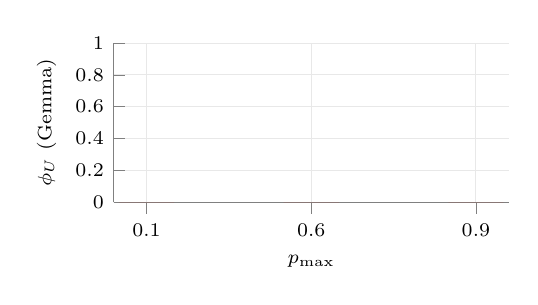
\begin{tikzpicture}
\pgfplotsset{raceaxis}
\begin{axis}[
  ybar, bar width=0.7cm,
  width=6.6cm, height=3.6cm,
  symbolic x coords={0.1,0.6,0.9},
  xtick=data, xlabel={$p_{\max}$},
  ylabel={$\phi_U$ (Gemma)}, ymax=1,
]
\addplot[fill=highlight,draw=none] coordinates {(0.1,0.000) (0.6,0.000) (0.9,0.000)};
\end{axis}
\end{tikzpicture}
\vspace{0.4em}
\begin{exampleblock}{Hai giả thuyết chưa phân biệt được}
\scriptsize
\textbf{(A)} Gemma hiểu trò chơi, kết luận Safe tối ưu.\\
\textbf{(B)} Gemma từ chối token \texttt{UNSAFE} do safety-tuning.\\
\textit{Phép thử quyết định:} đổi nhãn thành \texttt{OPTION\_A/B}.
\end{exampleblock}
\end{columns}
\end{frame}

\begin{frame}{Qwen2.5-14B: chuyển pha đúng vòng 5}
\centering
\begin{tikzpicture}
\pgfplotsset{raceaxis}
\begin{axis}[
  ybar, bar width=0.55cm,
  width=0.92\linewidth, height=4.6cm,
  xtick={1,2,3,4,5,6,7,8,9,10}, xlabel={Vòng},
  ylabel={Tỷ lệ Unsafe},
  ymax=0.8,
  legend style={font=\tiny,draw=none,fill=none,at={(0.5,-0.30)},anchor=north,legend columns=-1},
  nodes near coords, nodes near coords style={font=\tiny},
]
\addplot[fill=skyblue,draw=none] coordinates {(1,0.00)(2,0.00)(3,0.00)(4,0.00)};
\addlegendentry{Safe tuyệt đối (vòng 1--4)}
\addplot[fill=accent,draw=none] coordinates {(5,0.283)(6,0.521)(7,0.354)(8,0.690)(9,0.194)(10,0.583)};
\addlegendentry{Sau \texttt{minRounds=5}}
\draw[deepblue,dashed,thick] (axis cs:4.5,0) -- (axis cs:4.5,0.8);
\end{axis}
\end{tikzpicture}
\begin{exampleblock}{Diễn giải}
\small Safe tuyệt đối ở cả 30 race trong vòng 1--4 (36\% mẫu panel, tất định hoàn toàn), bật Unsafe đúng từ vòng 5 --- vòng đầu tiên race \textbf{có thể} kết thúc. Qwen đang đọc luật dừng và chơi endgame có lý.
\end{exampleblock}
\end{frame}

\begin{frame}{Bị dẫn trước $\Rightarrow$ Unsafe mạnh --- tái tạo đúng phát hiện trung tâm của paper}
\centering
\begin{tikzpicture}
\pgfplotsset{raceaxis}
\begin{axis}[
  ybar, bar width=6pt, width=0.92\linewidth, height=4.4cm,
  symbolic x coords={0.1,0.6,0.9}, xtick=data, xlabel={$p_{\max}$},
  ylabel={$\phi_U$}, ymax=1.05,
  enlarge x limits=0.25,
  legend style={font=\tiny,draw=none,fill=none,at={(0.5,-0.30)},anchor=north,legend columns=-1},
]
\addplot[fill=skyblue,draw=none] coordinates {(0.1,0.385)(0.6,0.125)(0.9,0.300)};
\addlegendentry{Dẫn trước (+0,5)}
\addplot[fill=gray,draw=none] coordinates {(0.1,0.157)(0.6,0.123)(0.9,0.137)};
\addlegendentry{Hòa (0,0)}
\addplot[fill=accent,draw=none] coordinates {(0.1,0.769)(0.6,0.938)(0.9,0.800)};
\addlegendentry{Bị dẫn (--0,5)}
\end{axis}
\end{tikzpicture}
\begin{alertblock}{Chênh lệch bị-dẫn trừ dẫn-trước}
\small \bad{+0,38} / \bad{+0,81} / \bad{+0,50} --- nhất quán và lớn ở cả ba treatment. Đúng phát hiện trung tâm của Fernández Domingos \& Han (2026).
\end{alertblock}
\end{frame}

\begin{frame}{Chia lượt, không phải quán tính --- ma trận chuyển trạng thái (vòng $\geq$5)}
\centering
\renewcommand{\arraystretch}{2.2}
\begin{tabular}{@{}l|cc@{}}
own $\backslash$ opp$_{t-1}$ & \textbf{Safe} & \textbf{Unsafe} \\
\hline
\textbf{Safe} & \cellcolor{skyblue!35}\shortstack{0,404\\{\tiny n=146}} & \cellcolor{accent!85}\shortstack{\textbf{0,892}\\{\tiny n=65}} \\
\textbf{Unsafe} & \cellcolor{skyblue!12}\shortstack{0,154\\{\tiny n=65}} & \cellcolor{skyblue!4}\shortstack{\textbf{0,048}\\{\tiny n=42}} \\
\end{tabular}
\vspace{0.4em}
\begin{exampleblock}{Đọc ma trận}
\small Đối thủ vừa Unsafe, mình vừa Safe $\Rightarrow$ \hl{89,2\%} mình chuyển Unsafe. Nhưng mình vừa Unsafe xong $\Rightarrow$ gần như chắc chắn lui về Safe (\hl{4,8\%}). \textbf{Chia lượt}, không phải momentum.
\end{exampleblock}
\end{frame}

\begin{frame}{Hệ số hồi quy Qwen (đặc tả 2, N=498, 10 cluster)}
\centering
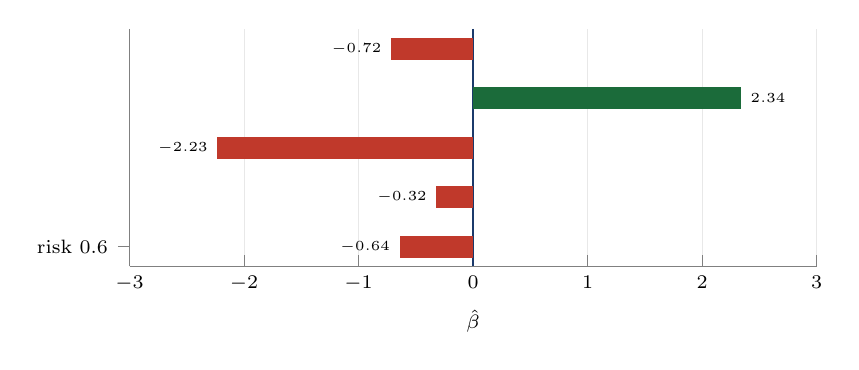
\begin{tikzpicture}
\pgfplotsset{raceaxisbar}
\begin{axis}[
  xbar, bar width=8pt,
  width=0.85\linewidth, height=4.6cm,
  symbolic y coords={ΔS (progress gap),opponent(t-1)=U,own(t-1)=U,risk 0.9,risk 0.6},
  ytick=data, y dir=reverse,
  xlabel={$\hat\beta$}, xmin=-3, xmax=3,
  ymajorgrids=false,
  extra x ticks={0}, extra x tick labels={},
  extra x tick style={grid=major,grid style={deepblue,thick},major tick length=0pt},
  nodes near coords, nodes near coords style={font=\tiny},
]
\addplot[xbar,fill=highlight,draw=none] coordinates {(-0.642,{risk 0.6})};
\addplot[xbar,fill=highlight,draw=none] coordinates {(-0.320,{risk 0.9})};
\addplot[xbar,fill=highlight,draw=none] coordinates {(-2.234,{own(t-1)=U})};
\addplot[xbar,fill=proposegreen,draw=none] coordinates {(2.339,{opponent(t-1)=U})};
\addplot[xbar,fill=highlight,draw=none] coordinates {(-0.717,{ΔS (progress gap)})};
\end{axis}
\end{tikzpicture}
\begin{alertblock}{Cẩn thận}
\scriptsize Chỉ 10 CRN cluster $\Rightarrow$ SE lạc quan. Đọc dấu/độ lớn như tín hiệu, không phải ước lượng chắc chắn. $\text{own}_{t-1}$ \bad{trái ngược} paper (paper: "không dự báo").
\end{alertblock}
\end{frame}

\section{Frontier: họ Gemini}

\begin{frame}{$\phi_U$ theo rủi ro --- Gemini giảm đơn điệu mạnh, ngược người}
\centering
\begin{tikzpicture}
\pgfplotsset{raceaxis}
\begin{axis}[
  width=0.86\linewidth, height=4.6cm,
  symbolic x coords={0.1,0.6,0.9}, xtick=data, xlabel={$p_{\max}$},
  ylabel={$\phi_U$}, ymax=1.05,
  legend style={font=\tiny,draw=none,fill=none,at={(0.5,-0.30)},anchor=north,legend columns=-1},
]
\addplot[gray,dashed,thick,mark=*,mark options={fill=gray}] coordinates {(0.1,0.64)(0.6,0.56)(0.9,0.56)};
\addlegendentry{Người (paper, tham chiếu)}
\addplot[skyblue,thick,mark=*,mark options={fill=skyblue}] coordinates {(0.1,1.000)(0.6,0.723)(0.9,0.539)};
\addlegendentry{gemini-3-flash-preview}
\addplot[accent,thick,mark=square*,mark options={fill=accent}] coordinates {(0.1,1.000)(0.6,0.801)(0.9,0.699)};
\addlegendentry{gemini-3.1-flash-lite}
\addplot[highlight,thick,mark=triangle*,mark options={fill=highlight}] coordinates {(0.1,0.838)(0.6,0.708)(0.9,0.626)};
\addlegendentry{gemini-3.5-flash-lite}
\end{axis}
\end{tikzpicture}
\begin{alertblock}{Ngược hướng với null quan trọng nhất của paper}
\small Người: 0,6 vs 0,9 không khác nhau (H1.2 bị bác bỏ). Cả ba Gemini: \bad{có ý nghĩa thống kê} (d = 1,03--1,87, p$<$0,01) --- và bão hòa gần 1,0 ở risk=0,1.
\end{alertblock}
\end{frame}

\begin{frame}{Persona: risk-averse khóa cứng, "adversarial" không đơn điệu}
\centering
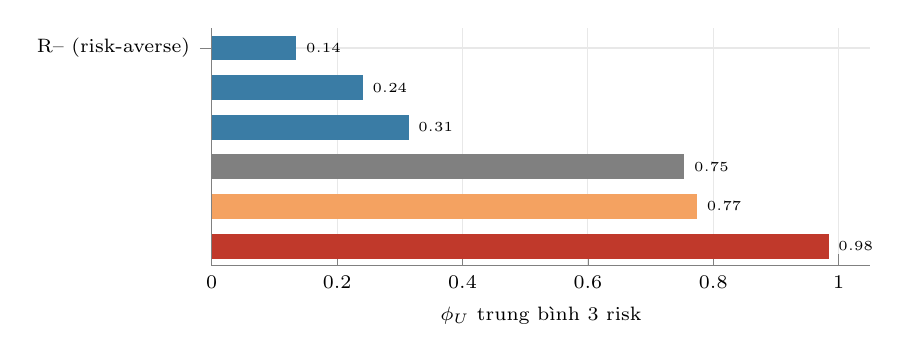
\begin{tikzpicture}
\pgfplotsset{raceaxisbar}
\begin{axis}[
  xbar, bar width=9pt,
  width=0.82\linewidth, height=4.6cm,
  symbolic y coords={S\_AA (2 ghế adversarial),R0 trung lập,Baseline,S\_CA (ghế coop.),S\_AC (ghế adv.),R-- (risk-averse)},
  ytick=data, xlabel={$\phi_U$ trung bình 3 risk}, xmin=0, xmax=1.05,
  nodes near coords, nodes near coords style={font=\tiny},
]
\addplot[xbar,fill=skyblue,draw=none] coordinates {(0.135,{R-- (risk-averse)})};
\addplot[xbar,fill=skyblue,draw=none] coordinates {(0.241,{S\_AC (ghế adv.)})};
\addplot[xbar,fill=skyblue,draw=none] coordinates {(0.314,{S\_CA (ghế coop.)})};
\addplot[xbar,fill=gray,draw=none] coordinates {(0.754,{Baseline})};
\addplot[xbar,fill=accent,draw=none] coordinates {(0.774,{R0 trung lập})};
\addplot[xbar,fill=highlight,draw=none] coordinates {(0.984,{S\_AA (2 ghế adversarial)})};
\end{axis}
\end{tikzpicture}
\begin{exampleblock}{Nghịch lý}
\small \texttt{S\_AC} (ghế "adversarial" nhưng đối thủ cooperative) lại \hl{thấp hơn} cả \texttt{S\_CA}. Chỉ mô tả thô --- mỗi persona chạy ở một protocol signature riêng, không tách được khỏi nhiễu batch.
\end{exampleblock}
\end{frame}

\begin{frame}{Hồi quy panel Gemini (đặc tả 6, N=2.814, 30 cluster)}
\centering
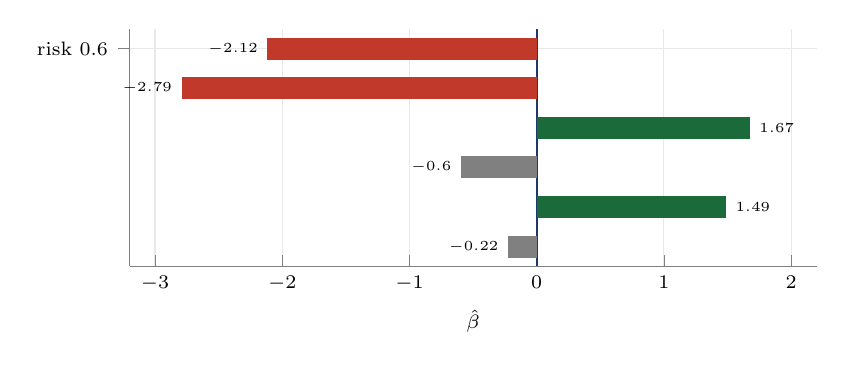
\begin{tikzpicture}
\pgfplotsset{raceaxisbar}
\begin{axis}[
  xbar, bar width=8pt,
  width=0.85\linewidth, height=4.6cm,
  symbolic y coords={ΔS (progress gap),opponent(t-1)=U,own(t-1)=U,Unsafe vòng 1,risk 0.9,risk 0.6},
  ytick=data, xlabel={$\hat\beta$}, xmin=-3.2, xmax=2.2,
  extra x ticks={0}, extra x tick labels={},
  extra x tick style={grid=major,grid style={deepblue,thick},major tick length=0pt},
  nodes near coords, nodes near coords style={font=\tiny},
]
\addplot[xbar,fill=highlight,draw=none] coordinates {(-2.116,{risk 0.6})};
\addplot[xbar,fill=highlight,draw=none] coordinates {(-2.791,{risk 0.9})};
\addplot[xbar,fill=proposegreen,draw=none] coordinates {(1.674,{Unsafe vòng 1})};
\addplot[xbar,fill=gray,draw=none] coordinates {(-0.595,{own(t-1)=U})};
\addplot[xbar,fill=proposegreen,draw=none] coordinates {(1.486,{opponent(t-1)=U})};
\addplot[xbar,fill=gray,draw=none] coordinates {(-0.224,{ΔS (progress gap)})};
\end{axis}
\end{tikzpicture}
\begin{exampleblock}{Khớp hướng người, nhưng mạnh hơn nhiều}
\small \good{opponent(t-1)}: người +0,607 $\to$ Gemini \good{+1,486} (gấp $\sim$2,4 lần). \good{Unsafe vòng 1}: người +0,217 (p$<$0,1) $\to$ Gemini +1,674 (p=0,001). Nhưng \bad{treatment} có ý nghĩa mạnh --- ngược paper.
\end{exampleblock}
\end{frame}

\begin{frame}{8 hiệu ứng người--LLM (E1--E8): 4/8 replicated}
\centering
\renewcommand{\arraystretch}{1}
\setlength{\tabcolsep}{3pt}
\begin{tabular}{cccc}
\chipcell{proposegreen!85}{\textbf{E1} opponent(t-1)}{replicated (mạnh hơn)} &
\chipcell{highlight!80}{\textbf{E2} $\Delta S$}{not replicated} &
\chipcell{proposegreen!85}{\textbf{E3} vòng 1}{replicated} &
\chipcell{highlight!80}{\textbf{E4} own(t-1)$\approx$0}{not replicated} \\[3pt]
\chipcell{highlight!80}{\textbf{E5} 0,6 vs 0,9 $\approx$0}{not replicated} &
\chipcell{proposegreen!85}{\textbf{E6} 0,1 vs 0,6}{replicated (d=3,08)} &
\chipcell{proposegreen!85}{\textbf{E7} $\phi_U$ tổng}{replicated (0,624)} &
\chipcell{highlight!80}{\textbf{E8} share AS}{not replicated} \\
\end{tabular}
\vspace{0.4em}
\begin{exampleblock}{Lưu ý về cách chấm}
\scriptsize "Replicated" chỉ xét \textbf{dấu} và ngưỡng ý nghĩa, không xét độ lớn có bằng người hay không. E1/E3/E6 "replicated" nhưng hệ số lớn hơn người 2--9 lần.
\end{exampleblock}
\end{frame}

\section{OpenAI: GPT-5-nano / GPT-5.4-nano}

\begin{frame}{$\phi_U$ theo rủi ro --- hình chữ U, không đơn điệu}
\centering
\begin{tikzpicture}
\pgfplotsset{raceaxis}
\begin{axis}[
  width=0.86\linewidth, height=4.6cm,
  symbolic x coords={0.1,0.6,0.9}, xtick=data, xlabel={$p_{\max}$},
  ylabel={$\phi_U$}, ymax=1.05,
  legend style={font=\tiny,draw=none,fill=none,at={(0.5,-0.30)},anchor=north,legend columns=-1},
]
\addplot[gray,dashed,thick,mark=*,mark options={fill=gray}] coordinates {(0.1,0.64)(0.6,0.56)(0.9,0.56)};
\addlegendentry{Người (tham chiếu)}
\addplot[skyblue,thick,mark=*,mark options={fill=skyblue}] coordinates {(0.1,0.123)(0.6,0.151)(0.9,0.145)};
\addlegendentry{gpt-5-nano}
\addplot[accent,thick,mark=square*,mark options={fill=accent}] coordinates {(0.1,0.577)(0.6,0.496)(0.9,0.567)};
\addlegendentry{gpt-5.4-nano}
\end{axis}
\end{tikzpicture}
\begin{exampleblock}{Điểm trũng thật ở risk=0,6}
\small \texttt{gpt-5.4-nano}, mẫu t$\geq$2: 0,1$\leftrightarrow$0,6 (d=0,662, p=0,043) và 0,6$\leftrightarrow$0,9 (d=--0,689, p=0,036) \good{có ý nghĩa}; 0,1$\leftrightarrow$0,9 gần bằng nhau (p=0,86). Không bão hòa gần 1,0 như Gemini.
\end{exampleblock}
\end{frame}

\begin{frame}{Persona: thứ hạng nhất quán trên 2 model độc lập}
\centering
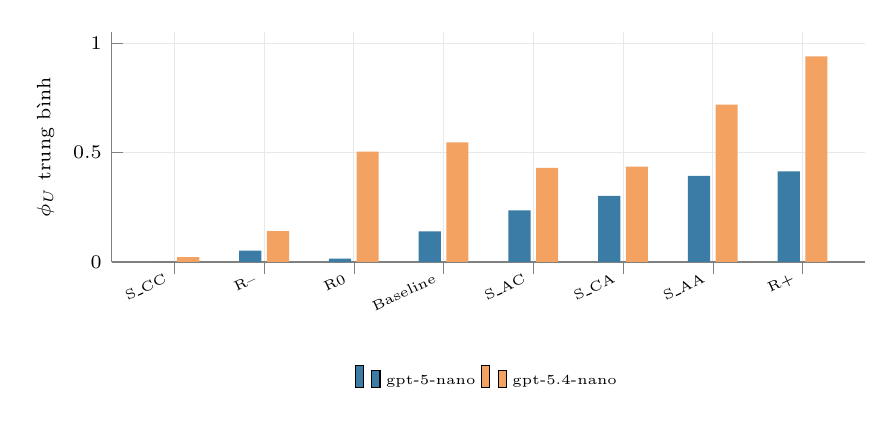
\begin{tikzpicture}
\pgfplotsset{raceaxis}
\begin{axis}[
  ybar, bar width=8pt,
  width=0.92\linewidth, height=4.5cm,
  symbolic x coords={S\_CC,R--,R0,Baseline,S\_AC,S\_CA,S\_AA,R+},
  xtick=data, x tick label style={rotate=25,anchor=east,font=\tiny},
  ylabel={$\phi_U$ trung bình}, ymax=1.05,
  legend style={font=\tiny,draw=none,fill=none,at={(0.5,-0.42)},anchor=north,legend columns=-1},
]
\addplot[fill=skyblue,draw=none] coordinates {(S\_CC,0.000)(R--,0.052)(R0,0.015)(Baseline,0.140)(S\_AC,0.236)(S\_CA,0.302)(S\_AA,0.394)(R+,0.414)};
\addlegendentry{gpt-5-nano}
\addplot[fill=accent,draw=none] coordinates {(S\_CC,0.022)(R--,0.141)(R0,0.504)(Baseline,0.547)(S\_AC,0.430)(S\_CA,0.436)(S\_AA,0.719)(R+,0.940)};
\addlegendentry{gpt-5.4-nano}
\end{axis}
\end{tikzpicture}
\begin{exampleblock}{Thứ hạng hợp lý nhất trong cả hai pilot}
\small R-- thấp nhất, R+ cao nhất, S\_CC$\approx$0. Nhưng \bad{gpt-5-nano sụp về Safe với BẤT KỲ persona nào}, kể cả R0 trung lập (0,14$\to$0,015) --- hiệu ứng "có persona hay không", không phải hướng persona.
\end{exampleblock}
\end{frame}

\begin{frame}{Ma trận rủi ro 6\texttimes6 (gpt-5.4-nano): mình chi phối, đối thủ bù trừ}
\centering
\renewcommand{\arraystretch}{1.6}
\setlength{\tabcolsep}{2pt}
{\small
\begin{tabular}{@{}r|cccccc@{}}
own$\backslash$opp & 1 & 2 & 3 & 4 & 5 & 6 \\
\hline
1 & \cellcolor{accent!0}{,002} & \cellcolor{accent!0}{,004} & \cellcolor{accent!0}{,002} & \cellcolor{accent!0}{,000} & \cellcolor{accent!1}{,008} & \cellcolor{accent!1}{,006} \\
2 & \cellcolor{accent!0}{,000} & \cellcolor{accent!0}{,000} & \cellcolor{accent!0}{,003} & \cellcolor{accent!1}{,006} & \cellcolor{accent!0}{,003} & \cellcolor{accent!0}{,002} \\
3 & \cellcolor{accent!48}{,479} & \cellcolor{accent!46}{,463} & \cellcolor{accent!39}{,385} & \cellcolor{accent!30}{,300} & \cellcolor{accent!25}{,252} & \cellcolor{accent!25}{,250} \\
4 & \cellcolor{accent!63}{,628} & \cellcolor{accent!58}{,581} & \cellcolor{accent!51}{,506} & \cellcolor{accent!45}{,446} & \cellcolor{accent!39}{,390} & \cellcolor{accent!35}{,345} \\
5 & \cellcolor{accent!83}{,833} & \cellcolor{accent!87}{,869} & \cellcolor{accent!83}{,834} & \cellcolor{accent!80}{,796} & \cellcolor{accent!73}{,729} & \cellcolor{accent!70}{,702} \\
6 & \cellcolor{accent!98}{\textbf{,982}} & \cellcolor{accent!98}{\textbf{,982}} & \cellcolor{accent!98}{\textbf{,983}} & \cellcolor{accent!99}{\textbf{,991}} & \cellcolor{accent!99}{\textbf{,985}} & \cellcolor{accent!99}{\textbf{,988}} \\
\end{tabular}}
\vspace{0.3em}
\begin{columns}[T]
\column{0.5\textwidth}
\begin{exampleblock}{Hàng: mức của MÌNH}
\scriptsize $\approx$0 (mức 1--2) $\to$ gần 1,0 (mức 6) --- \hl{dose-response} sạch hơn người (paper: không tìm thấy quan hệ nào).
\end{exampleblock}
\column{0.5\textwidth}
\begin{alertblock}{Cột: mức của ĐỐI THỦ}
\scriptsize Trong mỗi hàng, $\phi_U$ \bad{giảm dần} khi đối thủ "ưa rủi ro" hơn --- chiều bù trừ, khớp dấu âm của \texttt{opponent\_prev} ở slide sau.
\end{alertblock}
\end{columns}
\end{frame}

\begin{frame}{Hồi quy panel GPT-nano: \bad{đảo dấu hoàn toàn} --- phát hiện nổi bật nhất}
\centering
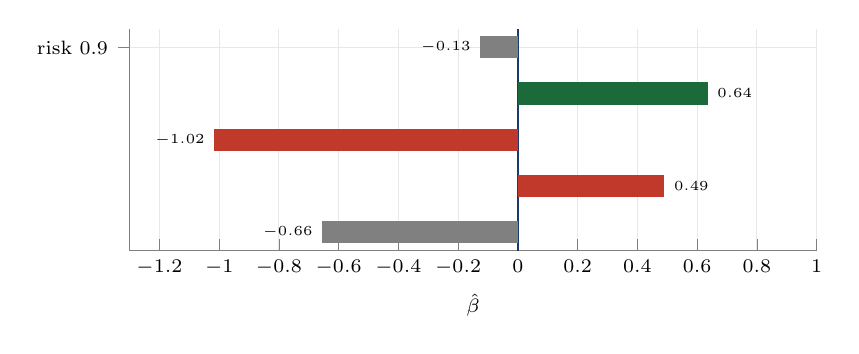
\begin{tikzpicture}
\pgfplotsset{raceaxisbar}
\begin{axis}[
  xbar, bar width=8pt,
  width=0.85\linewidth, height=4.4cm,
  symbolic y coords={own$\times$opp(t-1),ΔS (progress gap),opponent(t-1)=U,Unsafe vòng 1,risk 0.9},
  ytick=data, xlabel={$\hat\beta$}, xmin=-1.3, xmax=1.0,
  extra x ticks={0}, extra x tick labels={},
  extra x tick style={grid=major,grid style={deepblue,thick},major tick length=0pt},
  nodes near coords, nodes near coords style={font=\tiny},
]
\addplot[xbar,fill=gray,draw=none] coordinates {(-0.126,{risk 0.9})};
\addplot[xbar,fill=proposegreen,draw=none] coordinates {(0.635,{Unsafe vòng 1})};
\addplot[xbar,fill=highlight,draw=none] coordinates {(-1.016,{opponent(t-1)=U})};
\addplot[xbar,fill=highlight,draw=none] coordinates {(0.490,{ΔS (progress gap)})};
\addplot[xbar,fill=gray,draw=none] coordinates {(-0.655,{own$\times$opp(t-1)})};
\end{axis}
\end{tikzpicture}
\begin{alertblock}{Người: opp(t-1) \good{+0,607}, $\Delta S$ \good{--0,296} --- ở đây cả hai \bad{đảo dấu}}
\scriptsize \texttt{opponent\_prev}: \bad{--1,016} (phòng thủ, không leo thang). $\Delta S$: \bad{+0,490} (dẫn trước $\to$ củng cố, không bảo toàn). \textbf{Cảnh báo:} statsmodels báo \texttt{converged: False} cả 6 đặc tả (quasi-separation, 88 dummy protocol) --- đọc như tín hiệu thô.
\end{alertblock}
\end{frame}

\begin{frame}{8 hiệu ứng người--LLM (E1--E8): chỉ 2/8, và 2 cái đảo dấu}
\centering
\renewcommand{\arraystretch}{1}
\setlength{\tabcolsep}{3pt}
\begin{tabular}{cccc}
\chipcell{highlight!85}{\textbf{E1} opponent(t-1)}{\textbf{đảo dấu}: --1,016} &
\chipcell{highlight!85}{\textbf{E2} $\Delta S$}{\textbf{đảo dấu}: +0,490} &
\chipcell{proposegreen!85}{\textbf{E3} vòng 1}{replicated} &
\chipcell{highlight!80}{\textbf{E4} own(t-1)$\approx$0}{not replicated} \\[3pt]
\chipcell{proposegreen!85}{\textbf{E5} 0,6 vs 0,9$\approx$0}{replicated} &
\chipcell{highlight!80}{\textbf{E6} 0,1 vs 0,6}{not replicated ($\approx$0)} &
\chipcell{highlight!80}{\textbf{E7} $\phi_U$ tổng}{not replicated (0,353)} &
\chipcell{highlight!80}{\textbf{E8} share AS}{not repl. (0,562)} \\
\end{tabular}
\begin{exampleblock}{Khác Gemini không chỉ ở \textit{số lượng} mà ở \textit{kiểu}}
\scriptsize Gemini "not replicated" vẫn đúng dấu. GPT-nano ở E1/E2 \bad{đảo dấu hoàn toàn}. Bảng gộp 44 cell rất không đồng nhất --- đọc như trung bình thô.
\end{exampleblock}
\end{frame}

\section{N-player (N=3): Qwen2.5-14B}

\begin{frame}{$\phi_U$ giảm theo rủi ro (69\%$\to$57\%$\to$47\%), p$<$0,001}
\centering
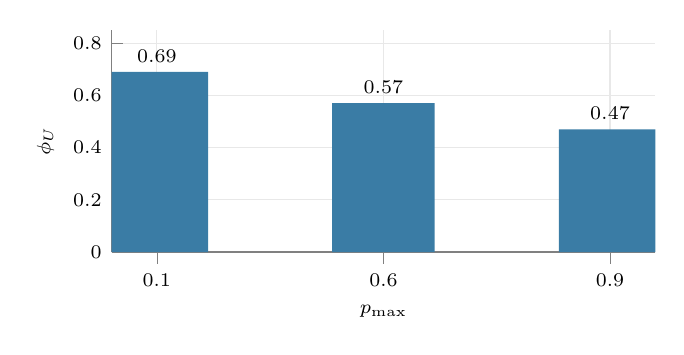
\begin{tikzpicture}
\pgfplotsset{raceaxis}
\begin{axis}[
  ybar, bar width=1.3cm,
  width=0.7\linewidth, height=4.4cm,
  symbolic x coords={0.1,0.6,0.9}, xtick=data, xlabel={$p_{\max}$},
  ylabel={$\phi_U$}, ymax=0.85,
  nodes near coords, nodes near coords style={font=\scriptsize},
]
\addplot[fill=skyblue,draw=none] coordinates {(0.1,0.69)(0.6,0.57)(0.9,0.47)};
\end{axis}
\end{tikzpicture}
\begin{exampleblock}{So với lý thuyết quần thể}
\small Kể cả sau khi \hl{quét $\beta$} tìm điểm khớp tốt nhất (chặt hơn cách cố định 2 điểm của frontier), lý thuyết vẫn dự báo \bad{dốc giảm mạnh hơn} thực tế ở risk 0,6/0,9.
\end{exampleblock}
\end{frame}

\begin{frame}{Persona Eckel-Grossman lấn át hoàn toàn tín hiệu rủi ro thực}
\centering
\begin{tikzpicture}[scale=1]
\draw[gray,thick] (0,0) -- (9,0) node[right,font=\scriptsize]{mức persona R1$\to$R6};
\draw[gray,thick] (0,0) -- (0,3.3) node[above,font=\scriptsize]{$\phi_U$};
\draw[highlight,thick] (0.5,0.15) -- (2.5,0.15) -- (2.5,3) -- (4.5,3) -- (4.5,0.15) -- (6.5,0.15) -- (6.5,3) -- (8.5,3);
\node[font=\tiny,highlight] at (4.5,-0.35) {5/6 mức: bậc thang $\approx$0\%\,/\,100\%};
\node[skyblue,circle,fill=skyblue,minimum size=4pt,inner sep=0pt] at (1.5,0.9) {};
\node[font=\tiny,skyblue,align=center] at (1.5,1.4) {riêng mức\\"trung tính"\\vẫn nhạy $p_{\max}$ thật};
\end{tikzpicture}
\begin{alertblock}{Đọc cẩn thận}
\small Sơ đồ minh họa định tính (không phải số đo chính xác từng mức). Chỉ \hl{2 race/ô} --- không đưa vào hồi quy được, cần xác nhận lại bằng confirmatory run.
\end{alertblock}
\end{frame}

\section{Tổng hợp xuyên mô hình}

\begin{frame}{Từ 4 mảnh rời rạc đến một câu hỏi chung}
\centering
\begin{tikzpicture}[
  font=\footnotesize,
  scatter/.style={rectangle, rounded corners=3pt, draw=highlight, fill=highlight!8,
    text width=3.0cm, align=center, inner sep=6pt},
  unified/.style={rectangle, rounded corners=3pt, draw=proposegreen, fill=proposegreen!10,
    text width=3.6cm, align=center, inner sep=8pt},
  flow/.style={-{Stealth[length=3mm]}, line width=1pt, accent}
]
\node[scatter] (a) {\bad{Baseline}\\Gemma: 0.000\\Qwen: chia lượt};
\node[scatter,below=6pt of a] (b) {\bad{Frontier}\\Gemini: giảm đơn điệu};
\node[scatter,below=6pt of b] (c) {\bad{OpenAI}\\GPT-nano: hình U, đảo dấu};
\node[scatter,below=6pt of c] (d) {\bad{N-player}\\persona $\gg$ risk thật};
\node[unified,right=2.2cm of b,yshift=-0.9cm] (e) {\good{Có tồn tại một\\"hành vi LLM" chung\\khi đối mặt rủi ro?}};
\draw[flow] (a) -- (e); \draw[flow] (b) -- (e); \draw[flow] (c) -- (e); \draw[flow] (d) -- (e);
\end{tikzpicture}
\begin{exampleblock}{Câu trả lời sơ bộ: không}
\small Bốn pilot tổng hợp tiếp theo cho thấy \textbf{hình dạng} và thậm chí \textbf{dấu} của hiệu ứng thay đổi theo từng model.
\end{exampleblock}
\end{frame}

\begin{frame}{$\phi_U(risk)$ không cùng hình dạng giữa các nguồn}
\centering
\begin{tikzpicture}
\pgfplotsset{raceaxis}
\begin{axis}[
  width=0.9\linewidth, height=4.6cm,
  symbolic x coords={0.1,0.6,0.9}, xtick=data, xlabel={$p_{\max}$},
  ylabel={$\phi_U$}, ymax=1.0,
  legend style={font=\tiny,draw=none,fill=none,at={(0.5,-0.32)},anchor=north,legend columns=3},
]
\addplot[gray,dashed,thick,mark=*,mark options={fill=gray}] coordinates {(0.1,0.64)(0.6,0.56)(0.9,0.56)};
\addlegendentry{Người (phẳng)}
\addplot[skyblue,thick,mark=square*,mark options={fill=skyblue}] coordinates {(0.1,0.946)(0.6,0.744)(0.9,0.621)};
\addlegendentry{Gemini (TB 3 model, giảm dốc)}
\addplot[accent,thick,mark=triangle*,mark options={fill=accent}] coordinates {(0.1,0.350)(0.6,0.324)(0.9,0.356)};
\addlegendentry{GPT-nano (TB 2 model, chữ U)}
\addplot[highlight,thick,mark=diamond*,mark options={fill=highlight}] coordinates {(0.1,0.239)(0.6,0.173)(0.9,0.196)};
\addlegendentry{Qwen 2-player}
\addplot[proposegreen,thick,mark=*,mark options={fill=proposegreen}] coordinates {(0.1,0.69)(0.6,0.57)(0.9,0.47)};
\addlegendentry{Qwen 3-player}
\end{axis}
\end{tikzpicture}
\begin{exampleblock}{Không có "hành vi LLM" phổ quát}
\small 5 đường, 5 hình dạng khác nhau: phẳng, dốc đơn điệu, chữ U, thấp-ổn định, giảm nhẹ. Chọn model là chọn cả một \textbf{hình dạng hành vi}, không chỉ một con số trung bình.
\end{exampleblock}
\end{frame}

\begin{frame}{Dấu hệ số \texttt{opponent\_prev} và $\Delta S$ đảo chiều theo model}
\centering
\begin{columns}[T]
\column{0.5\textwidth}
\centering{\scriptsize\bfseries opponent(t-1) = Unsafe}
\begin{tikzpicture}
\pgfplotsset{raceaxisbar}
\begin{axis}[
  xbar, bar width=8pt,
  width=\linewidth, height=4.3cm,
  symbolic y coords={Qwen 3p (+1.472),Qwen 2p (+2.339),GPT-nano (--1.016),Gemini (+1.486),Người (+0.607)},
  ytick=data, y tick label style={font=\tiny}, xlabel={$\hat\beta$},
  xmin=-1.5, xmax=2.8,
  extra x ticks={0}, extra x tick labels={},
  extra x tick style={grid=major,grid style={deepblue,thick},major tick length=0pt},
]
\addplot[xbar,fill=deepblue,draw=none] coordinates {(0.607,{Người (+0.607)})};
\addplot[xbar,fill=proposegreen,draw=none] coordinates {(1.486,{Gemini (+1.486)})};
\addplot[xbar,fill=highlight,draw=none] coordinates {(-1.016,{GPT-nano (--1.016)})};
\addplot[xbar,fill=proposegreen,draw=none] coordinates {(2.339,{Qwen 2p (+2.339)})};
\addplot[xbar,fill=proposegreen,draw=none] coordinates {(1.472,{Qwen 3p (+1.472)})};
\end{axis}
\end{tikzpicture}
\column{0.5\textwidth}
\centering{\scriptsize\bfseries ΔS (progress gap before)}
\begin{tikzpicture}
\pgfplotsset{raceaxisbar}
\begin{axis}[
  xbar, bar width=8pt,
  width=\linewidth, height=4.3cm,
  symbolic y coords={Qwen 3p ($\approx$0 n.s.),Qwen 2p (--0.717),GPT-nano (+0.490),Gemini (--0.224 n.s.),Người (--0.296)},
  ytick=data, y tick label style={font=\tiny}, xlabel={$\hat\beta$},
  xmin=-1.0, xmax=0.7,
  extra x ticks={0}, extra x tick labels={},
  extra x tick style={grid=major,grid style={deepblue,thick},major tick length=0pt},
]
\addplot[xbar,fill=deepblue,draw=none] coordinates {(-0.296,{Người (--0.296)})};
\addplot[xbar,fill=proposegreen,draw=none] coordinates {(-0.224,{Gemini (--0.224 n.s.)})};
\addplot[xbar,fill=highlight,draw=none] coordinates {(0.490,{GPT-nano (+0.490)})};
\addplot[xbar,fill=proposegreen,draw=none] coordinates {(-0.717,{Qwen 2p (--0.717)})};
\addplot[xbar,fill=gray,draw=none] coordinates {(0.032,{Qwen 3p ($\approx$0 n.s.)})};
\end{axis}
\end{tikzpicture}
\end{columns}
\begin{alertblock}{Ảnh quan trọng nhất của đợt này}
\scriptsize \good{Xanh} = cùng dấu người. \bad{Đỏ} = đảo dấu. Chỉ GPT-nano đảo cả hai hiệu ứng trung tâm của paper gốc cùng lúc --- nhưng hồi quy đó \texttt{converged=False}, nên đọc như tín hiệu thô, chưa kết luận.
\end{alertblock}
\end{frame}

\begin{frame}{Tỷ lệ tái tạo 8 hiệu ứng người: không model nào đầy đủ, không theo cùng một cách}
\centering
\begin{tikzpicture}
\pgfplotsset{raceaxis}
\begin{axis}[
  ybar, bar width=1.4cm,
  width=0.6\linewidth, height=4.4cm,
  symbolic x coords={Gemini,GPT-nano}, xtick=data,
  ylabel={Số hiệu ứng / 8}, ymax=8.6,
  nodes near coords,
]
\addplot[fill=proposegreen,draw=none] coordinates {(Gemini,4)(GPT-nano,2)};
\end{axis}
\end{tikzpicture}
\begin{exampleblock}{Khác nhau cả ở \textit{loại} không-khớp}
\small Gemini: 4 không-khớp đều là đúng dấu nhưng quá mạnh. GPT-nano: 6 không-khớp, trong đó \bad{2 cái đảo dấu hoàn toàn}. Không thể tổng quát hóa "LLM hành xử như người" hay ngay cả "LLM hành xử giống nhau".
\end{exampleblock}
\end{frame}

\section{Giới hạn \& việc cần làm tiếp}

\begin{frame}{Giới hạn cần giữ khi diễn giải}
\begin{columns}[T]
\column{0.49\textwidth}
\begin{alertblock}{Thống kê}
\small
\begin{itemize}\setlength\itemsep{2pt}
\item Tất cả \texttt{run\_phase = pilot}, chưa \texttt{confirmatory}.
\item OpenAI: hồi quy \bad{không hội tụ} (quasi-separation, 88 dummy protocol).
\item Baseline/nplayer: chỉ 10--20 CRN cluster --- SE lạc quan.
\item N-player persona: 2 race/ô, không đủ cho hồi quy.
\end{itemize}
\end{alertblock}
\column{0.49\textwidth}
\begin{alertblock}{Đo lường}
\small
\begin{itemize}\setlength\itemsep{2pt}
\item Persona \bad{confound với protocol/batch} ở cả frontier và openai --- 2 nguyên nhân cấu trúc khác nhau.
\item \texttt{first\_round\_unsafe} hằng số $\Rightarrow$ nhiều đặc tả hồi quy \textbf{singular}.
\item Gemma: 2 giả thuyết (A)/(B) chưa phân biệt được.
\end{itemize}
\end{alertblock}
\end{columns}
\vspace{0.4em}
\begin{exampleblock}{Nguyên tắc báo cáo}
\small Chỉ nói \textbf{tín hiệu pilot}; không dùng deck này làm bằng chứng cho bất kỳ RQ nào trong PROJECT.md.
\end{exampleblock}
\end{frame}

\begin{frame}{Việc cần làm tiếp}
\begin{enumerate}\small\setlength\itemsep{4pt}
\item \textbf{Phép thử đổi nhãn} \texttt{OPTION\_A/B} cho Gemma --- phân biệt giả thuyết (A) hiểu luật vs (B) từ chối từ.
\item \textbf{Tạo biến thiên vòng 1} (persona \texttt{risk\_seeking}/\texttt{adv\_adv}) để \texttt{first\_round\_unsafe} hết là hằng số.
\item \textbf{Chạy persona cùng session / qua \texttt{kaggle\_benchmarks}} để gỡ confound protocol.
\item \textbf{Mixed-effects logit} (TA.4) và \textbf{EGTtools} (TD.2) để mở khóa các mục đang thiếu.
\item \textbf{Khóa protocol} và đặt \texttt{RUN\_PHASE\_OVERRIDE=confirmatory} chỉ sau khi 4 bước trên xong.
\end{enumerate}
\vspace{0.4em}
\begin{exampleblock}{Thứ tự}
\small (1) và (2) chặn đường trước tiên --- chạy thêm repetition bây giờ chỉ nhân bản hai vấn đề này lên, không thêm thông tin.
\end{exampleblock}
\end{frame}

\section{Kết}

\begin{frame}[standout]
Bốn model, bốn hành vi khác nhau --- kể cả \bad{đảo dấu} hiệu ứng trung tâm của paper người.\\[8pt]
\small\color{accent} Chưa đủ confirmatory để kết luận --- nhưng đủ để không giả định LLM hành xử như người, hay giống nhau.
\end{frame}

\begin{frame}[standout]
Cảm ơn --- rất mong nhận được góp ý.
\end{frame}

\appendix

\begin{frame}{Backup 1 --- Hệ số hồi quy đầy đủ, cả 4 nguồn}
\centering
\scriptsize
\renewcommand{\arraystretch}{1.2}
\resizebox{\linewidth}{!}{%
\begin{tabular}{lccccc}
\toprule
Biến & Người & Gemini (spec 6) & GPT-nano (spec 6) & Qwen 2p (spec 2) & Qwen 3p (spec 3) \\
\midrule
opponent/others(t-1)=U & +0,607 (p=0,002) & +1,486 (p$<$0,001) & \bad{--1,016} (p$<$0,001) & +2,339 (p$<$0,001) & +1,472 (p$<$0,001) \\
own(t-1)=U & --0,193 (n.s.) & --0,595 (n.s.) & +0,170 (n.s.) & --2,234 (p$<$0,001) & +1,101 (p$<$0,001) \\
$\Delta S$ (progress gap) & --0,296 (p=0,048) & --0,224 (n.s.) & \bad{+0,490} (p$<$0,001) & --0,717 (p=0,013) & +0,032 (n.s.) \\
Unsafe vòng 1 & +0,217 (p$<$0,10) & +1,674 (p=0,001) & +0,635 (p$<$0,001) & không ước lượng được & hằng số \\
Pseudo R\textsuperscript{2} & 0,006--0,040 & 0,450 & 0,347 & 0,194 & --- \\
Hội tụ? & có & có & \bad{không} & có (spec 1--2) & có \\
\bottomrule
\end{tabular}}
\vspace{0.5em}
{\scriptsize Nguồn: \texttt{results/reports/baseline.md} \S4.4; \texttt{results/reports/frontier/report.md} \S4; \texttt{results/reports/openai/report.md} \S5; \texttt{results/reports/nplayer/derived/clustered\_logit\_coefficients.csv} spec 3.}
\end{frame}

\begin{frame}[fragile]{Backup 2 --- Provenance \& lệnh tái tạo}
\scriptsize
\begin{block}{4 file nguồn (không tính lại từ CSV thô)}
\texttt{results/reports/baseline.md} \textbullet\ \texttt{results/reports/frontier/report.md} \textbullet\ \texttt{results/reports/openai/report.md} \textbullet\ \texttt{results/reports/nplayer/report.md}
\end{block}
\begin{block}{Lệnh tái tạo (ví dụ openai)}
\begin{verbatim}
.venv-kaggle/bin/python3 results/scripts/analyze_ai_race.py \
  --input results/frontier/openai --output results/reports/openai/derived \
  --fit-logit --fit-logit-robustness \
  --allow-mixed-protocols --allow-nonfinal-runs \
  --allow-nonconfirmatory-runs --allow-missing-persona-condition
\end{verbatim}
\end{block}
\begin{alertblock}{Freeze before you look}
\small Mọi con số trên đây gắn với \texttt{run\_manifest.json} và \texttt{prompt\_sha256} đã khóa. Đổi prompt/config = \texttt{promptVersion} mới, không pool chung.
\end{alertblock}
\end{frame}

\begin{frame}{Tham chiếu chính}
\begin{beamercolorbox}[sep=.5cm,rounded=true]{normal text}
{\scriptsize\color{skyblue}\bfseries 2026 --- ARXIV:2607.26034}\par\vspace{.25cm}
{\large\bfseries Falling Behind Drives Unsafe Development\\in an Idealised AI Race Experiment}\par\vspace{.2cm}
{\normalsize E. Fernández Domingos \& T. A. Han}\par\vspace{.35cm}
{\color{skyblue}\texttt{https://arxiv.org/abs/2607.26034}}
\end{beamercolorbox}
\vspace{0.6em}
{\small\bfseries TÀI LIỆU DỰ ÁN}\par
{\color{gray}\small Engine, prompt, config, test và kết quả phân tích được lưu trong repo này (\texttt{CLAUDE.md}, \texttt{PROJECT.md}, \texttt{results/}).}
\end{frame}

\end{document}
